\documentclass[10pt,a4paper]{article}
\usepackage[a4paper, left=3cm, right=3cm, top=3cm, bottom=3cm, headsep=10mm, footskip=12mm]{geometry}
\usepackage[T1]{fontenc}
\usepackage[ngerman, english]{babel}    % mehrsprachiger Textsatz
% babel: letzte Sprache in Optionen zeigt die Sprache des Dokumentes
% und kann durch den Befehl \selectlanguage{} geaendert werden
% Passen Sie die Optionen des babel-Paketes nach Bedarf an!
\usepackage{float}
\usepackage{graphicx}
\usepackage{pdflscape}
\usepackage{mathtools}
\usepackage{amssymb, amsmath, amstext}
\usepackage{amsthm}
\usepackage{xcolor}
\usepackage{nameref}
\usepackage{siunitx}
\usepackage{makecell}
\usepackage{hyperref}
\usepackage{enumitem}
\usepackage[superscript,biblabel]{cite}
\usepackage{caption}
\usepackage{subcaption}
\usepackage{tabularx} 			% Tabellen erzeugen
\usepackage{multirow}			 % Zeilen in Tabellenbearbeitung
\usepackage{multicol} 			% Spalten in Tabellenbearbeitung 
\usepackage{lmodern}                        % Ersatz fuer Computer Modern-Schriften 
\usepackage{amsmath}                                           % zum besseren Aussehen am Bildschirm
\usepackage{booktabs} % für schönere Tabellen
\usepackage{sidecap}
\usepackage{rotating} % für die Landscape-Umgebung
\usepackage{afterpage}
\definecolor{Bluetitle}{HTML}{1F3864}
\definecolor{Greyish}{HTML}{5A5A5A}
\renewcommand{\refname}{Reference}
\usepackage{array,multirow}
\newcommand{\specialcell}[2][c]{%
	\begin{tabular}[#1]{@{}c@{}}#2\end{tabular}}




\begin{document}
	
	\begin{titlepage}
		\begin{center}
			\begin{figure}[h!tbp]
				
\includegraphics[width=\linewidth]{HUlogo.PNG}
			\end{figure}
			\vspace*{0.5cm}
			
			\textcolor{Bluetitle}{\textbf{\huge V2 Photosensitivitätsanalyse von Grünalgen C. reinhardtii}}\par
			
			\vspace*{1.4cm}
			
			\textcolor{Greyish}{\textbf{Versuchsdurchführende}}\par
			\textcolor{Greyish}{Tom Oberländer (633676)}\par
			\textcolor{Greyish}{Huyen Anh Nguyen (572309)}\par
			\vspace*{0.5cm}
			\textcolor{Greyish}{\textbf{Versuchsort}}\par
			\textcolor{Greyish}{Institut für Biophysik}\par
			\textcolor{Greyish}{Invalidenstr.42, Erdgeschoss rechts}\par
			\vspace*{0.5cm}
			\textcolor{Greyish}{\textbf{Versuchsbetreuer}}\par
			\textcolor{Greyish}{Yousef Kamrani}\par
			
			\vspace*{1.5 cm}
			
			\textcolor{Greyish}{07. März 2024}\par
			
			\vspace*{1.5 cm}
			
			
		\end{center}
		
	\tableofcontents
			
	\end{titlepage}
	
	
	\section{Einführung}
	
	Die Grünalge Chlamydomonas reinhardtii  (abgekürzt: C. reinhardtii) ist in der Lage mit ihren zwei Flagella sich fortzubewegen. Zudem besitzt die Grünalge ein Augenfleck, dass photosensitiv ist und somit Licht wahrnehmen kann.\\
	Eine durch Licht gerichtete Bewegung wird als Phototaxis bezeichnet und es gibt zwei große Unterscheidungen von Phototaxen. Es wird zwischen Phobo-Phototaxis, wobei die Bewegungsrichtung bei einer Veränderung der Strahlungsintensität nicht mit der Strahlungsrichtung korreliert und Tobo-Phototaxis, wo die Bewegungsrichtung mit der Strahlungsrichtung korreliert.\\
	Bei der Tobo-Phototaxis wird zudem noch zwischen negativen und positiven Tobo-Phototaxis unterschieden.\\
	Welche phototaktisches Verhalten wird bei C. reinhardtii beobachtet und bei welchen Wellenlänge wird die stärkste Reaktion gemessen?\\
	Der Versuch wird in drei Punkten gegliedert, um die Frage zu beantworten:
	\begin{itemize}
		\item  grobe Bestimmung der Bewegungsmuster bei grünes, blaues und rotes Licht unterm Fluoreszenzmikroskop
		\item photometrische quantitative Bestimmung des Aktionsspektrums der Grünalge bei der Wellenlänge $\lambda$ = 455, 470, 505, 530 nm
		\item mikroskopische Beobachtung des Verhalten der Grünalgen bei der Zugabe von 1 mol/L Salzsäure in das Medium
	\end{itemize}
	
	\section{Versuchsdurchführung}
	\subsection{Bewegungsmuster unterm Fluoreszenzmikroskop}
	Es wird 1 mL unverdünntes C. reinhardtii Suspension (Stockkonzentration beträgt 0.36 oD/mL in Nitrogen Minimal Medium kultiviert) in eine Mikroskop geeignete Küvette überführt und unterm Mikroskop die Bewegungsmuster begutachtet, ohne Lichteinfluss.\\
	Dann Wird die Bewegungsmuster für grünes, rotes und blaues Licht untersucht.
	
	\subsection{Photometrische Bestimmung des Aktionsspektrum}
	Für die photometrische Analyse wird die Kultur auf 1.1 oD/mL verdünnt. \\
	In einer Küvette wird die homogene Suspensionskultur überführt und bei der Wellenlänge $\lambda$ = 455, 470, 505, 530 nm photometrisch bei unterschiedlichen Lichtintensität von 0 - 100 $\%$ bestimmt.
	
	\subsection{pH-Veränderung des Medium}
	Es wird zu 3 mL unverdünnten Suspensionskultur 0.5 mL 1 M Salzsäure hinzugegeben und homogenisiert.\\
	Die Suspension wird in eine Mikroskopgeeignete Küvette überführt und unterm Mikroskop analysiert.

	\section{Ergebnis}
		\begin{figure}[H]
		\centering
		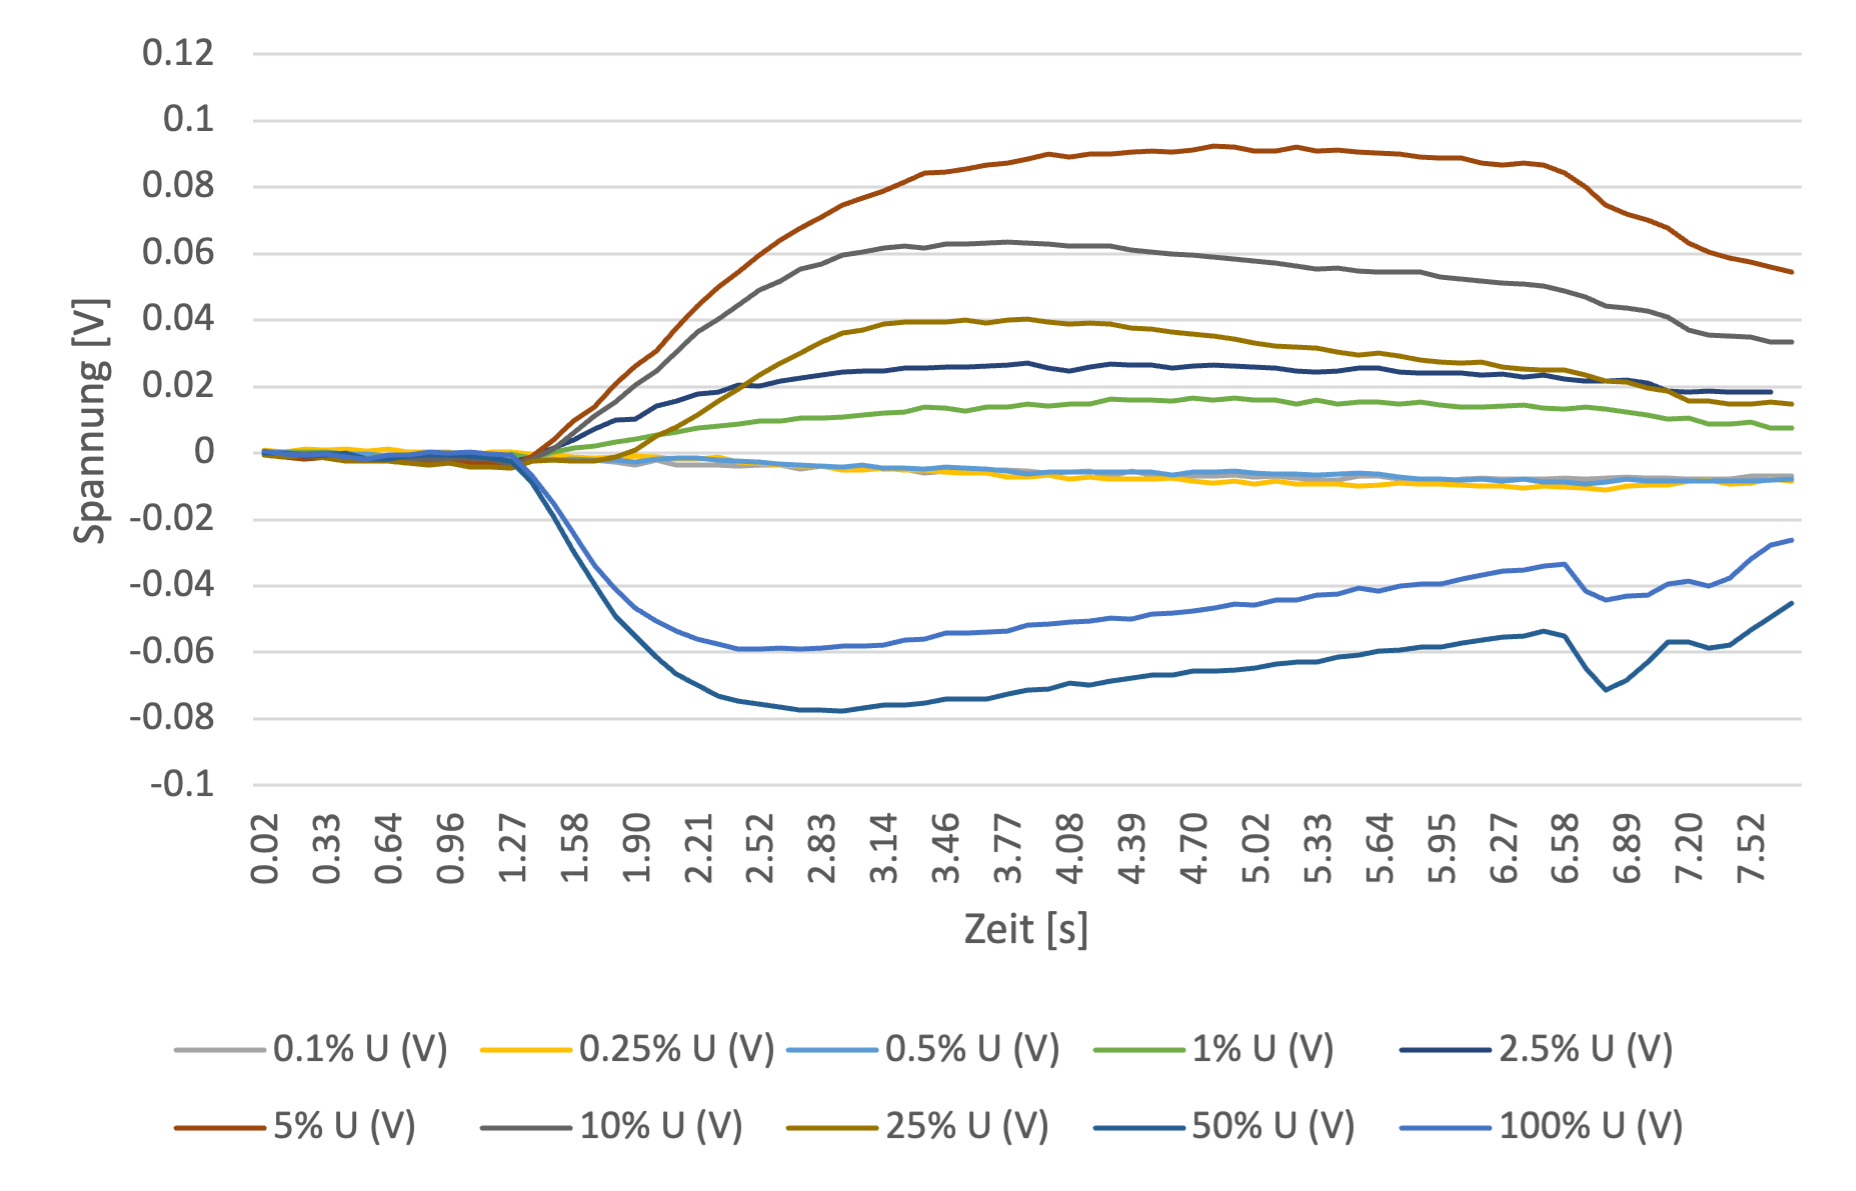
\includegraphics[scale=1]{Picture 1.png}
		\caption{Lichtstreukurven bei $\lambda$ = 455 nm für 10 verschiedenen Filtereinstellung die Abhängigkeit der Spannung mit der Zeit. }
		\label{fig:455nm}
	\end{figure}
	
		\begin{figure}[H]
		\centering
		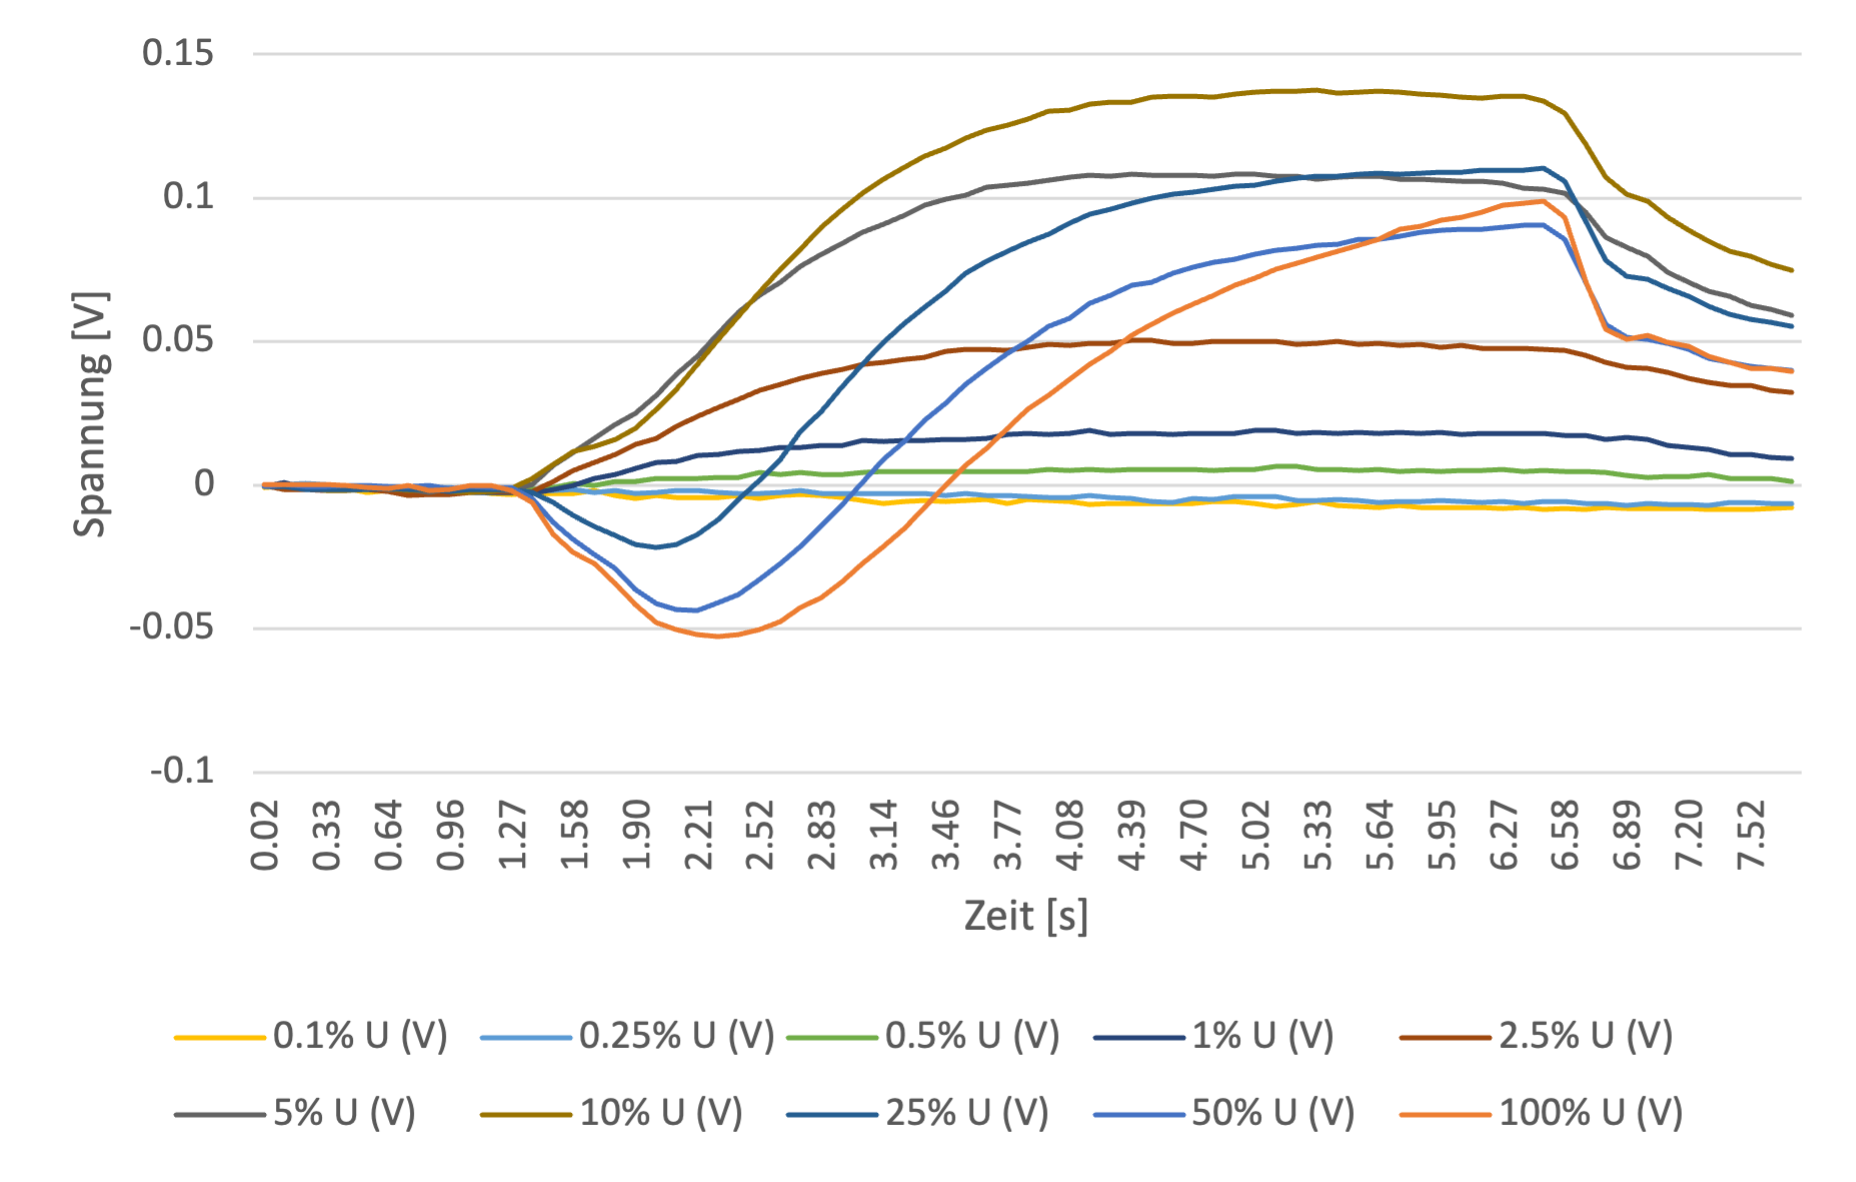
\includegraphics[scale=1]{Picture 2.png}
		\caption{Lichtstreukurven bei $\lambda$ = 470 nm für 10 verschiedenen Filtereinstellung die Abhängigkeit der Spannung mit der Zeit. }
		\label{fig:470nm}
	\end{figure}

	\begin{figure}[H]
	\centering
	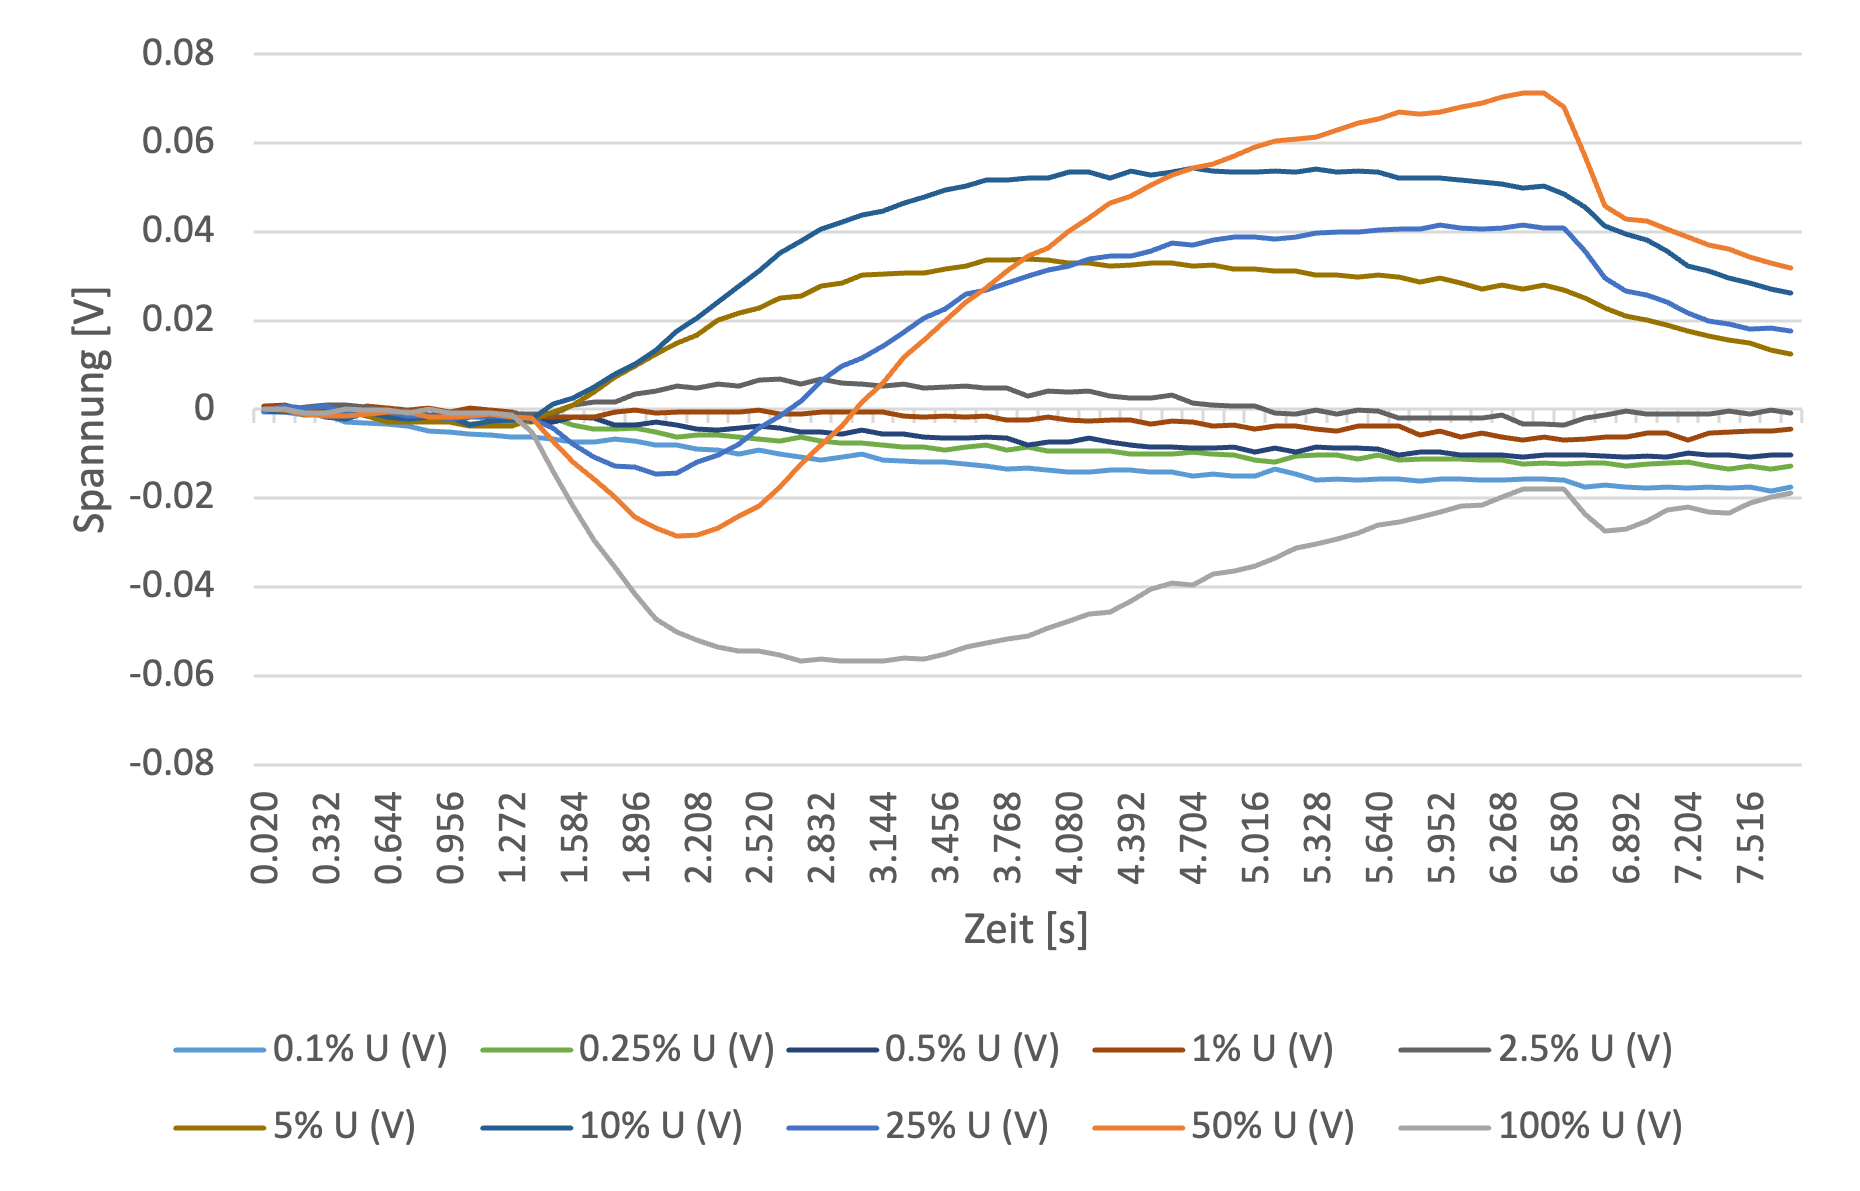
\includegraphics[scale=1]{Picture 3.png}
	\caption{Lichtstreukurven bei $\lambda$ = 505 nm für 10 verschiedenen Filtereinstellung die Abhängigkeit der Spannung mit der Zeit. }
	\label{fig:505nm}
	\end{figure}

	\begin{figure}[H]
	\centering
	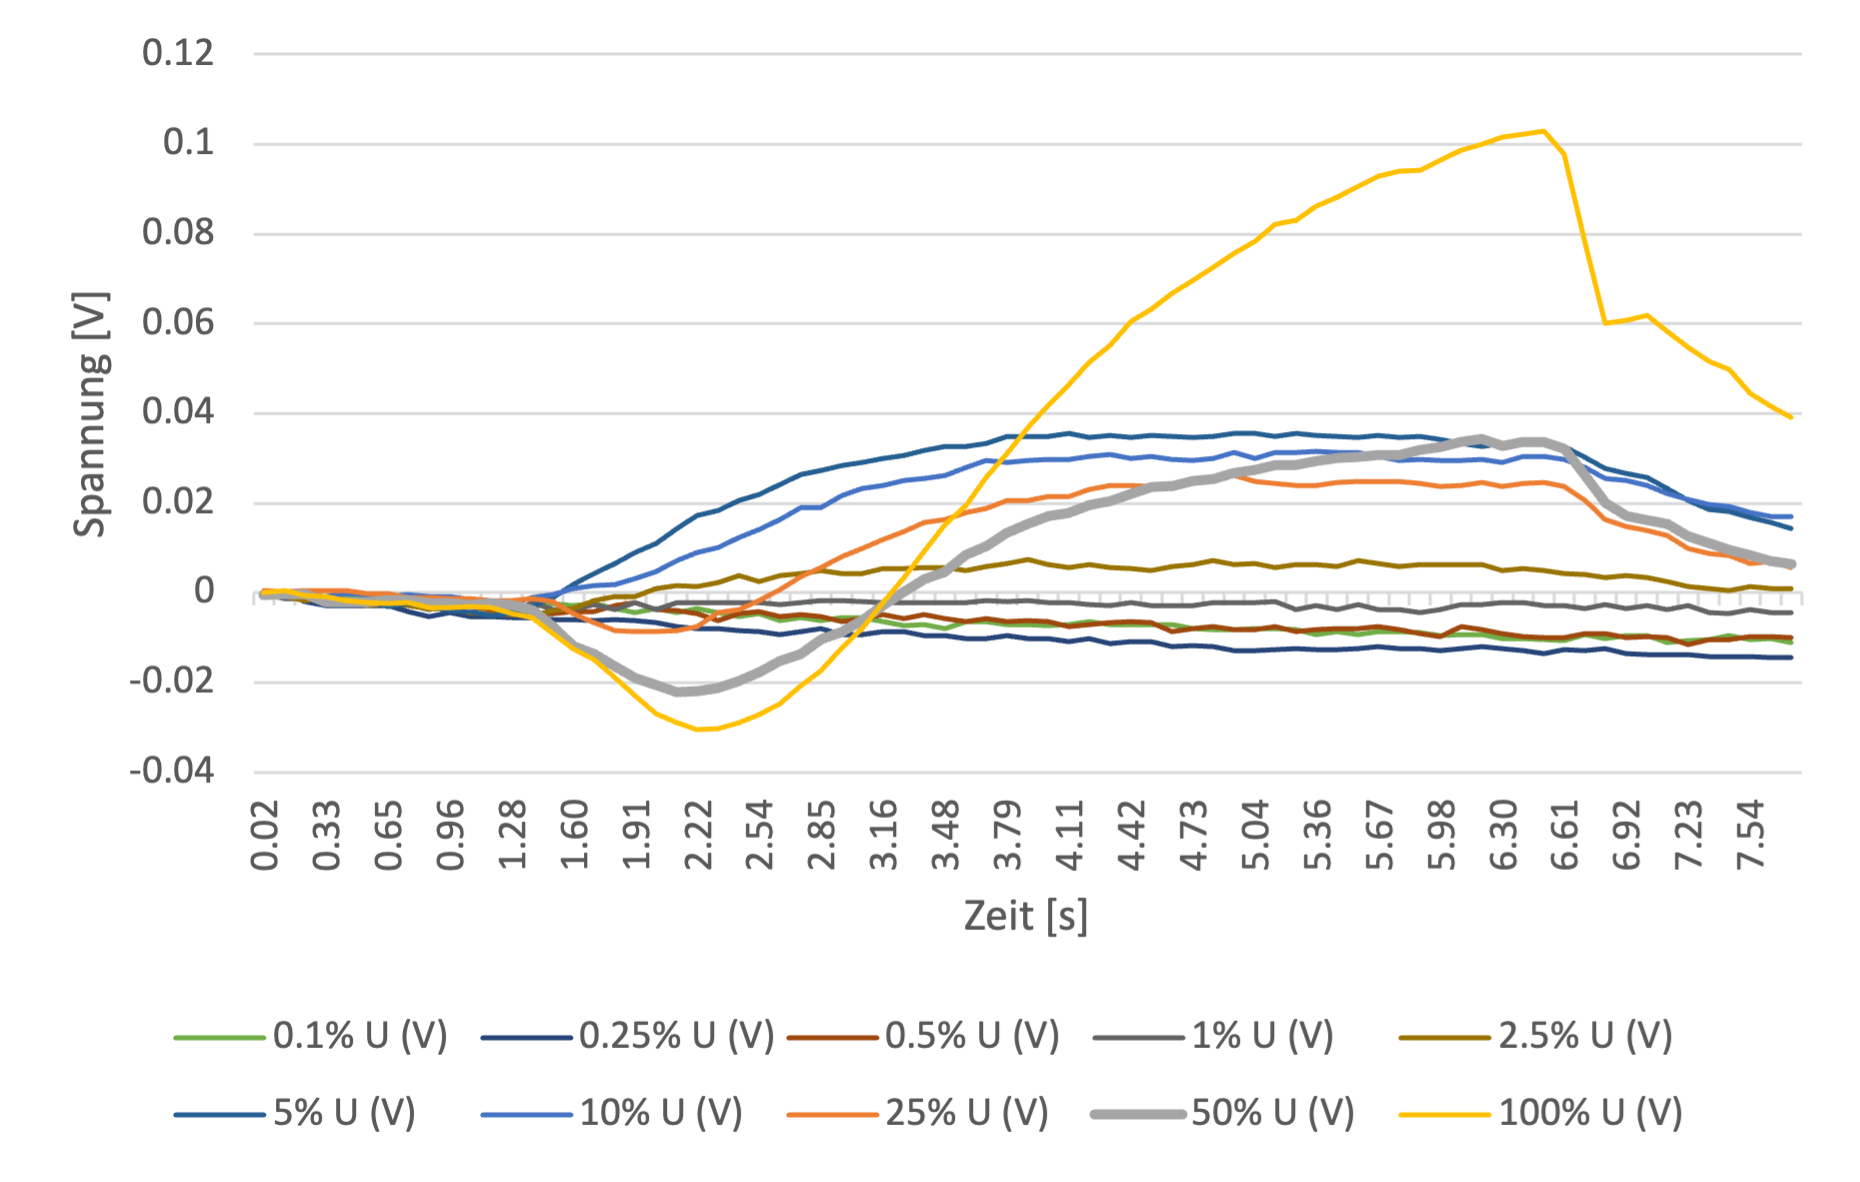
\includegraphics[scale=1]{Picture 4.png}
	\caption{Lichtstreukurven bei $\lambda$ = 530 nm für 10 verschiedenen Filtereinstellung die Abhängigkeit der Spannung mit der Zeit. }
	\label{fig:530nm}
	\end{figure}
	
		\begin{figure}[H]
		\centering
		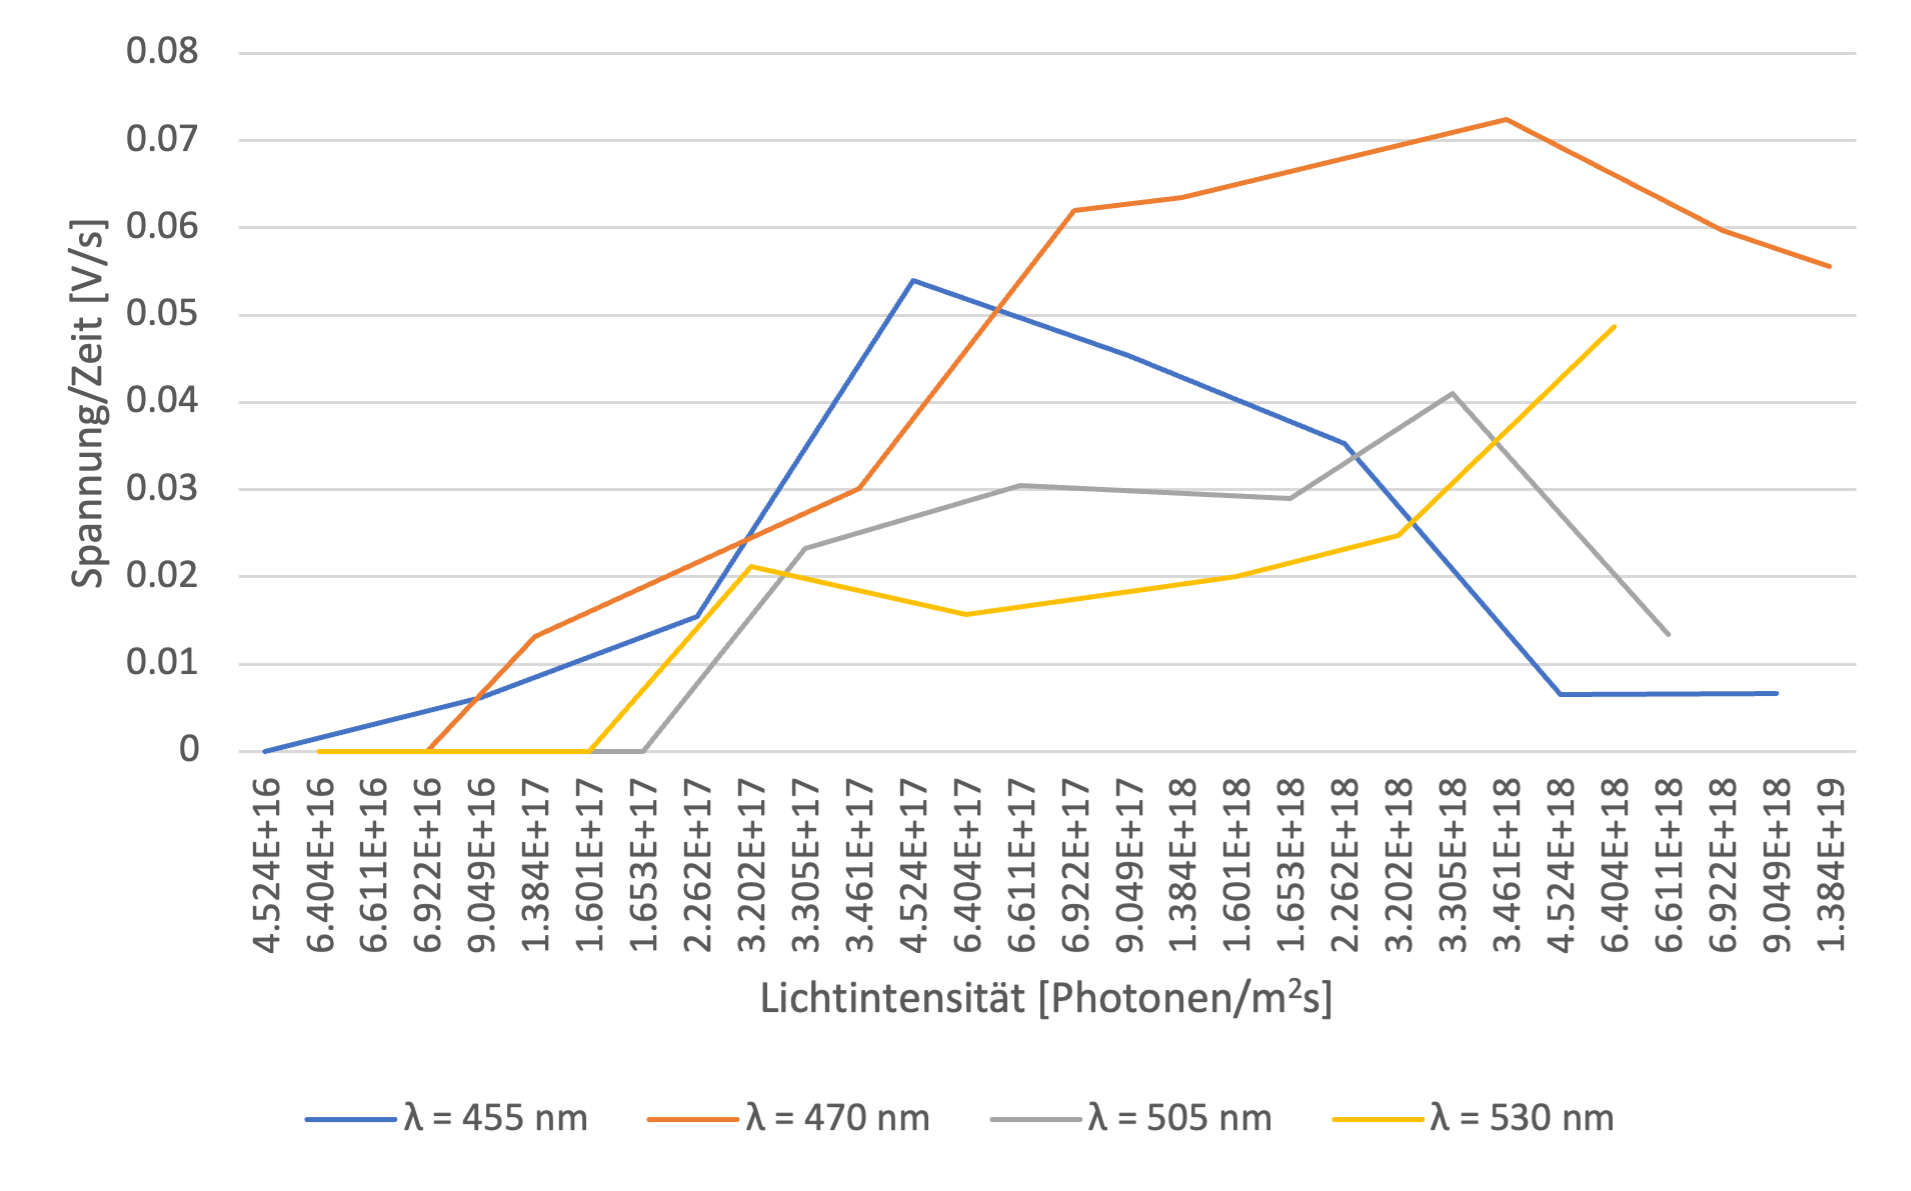
\includegraphics[scale=1]{Picture 5.png}
		\caption{Absorptionsspektrum von nativen eGFP und Puffer bei  $\lambda$ = 350-520 nm. \\
			Puffer dient hier als Referenzprobe\\
			Der Absorptionsmaxima liegt bei $\lambda$ = 490 nm.}
		\label{fig:Lichtitration}
	\end{figure}
	
		\begin{figure}[H]
		\centering
		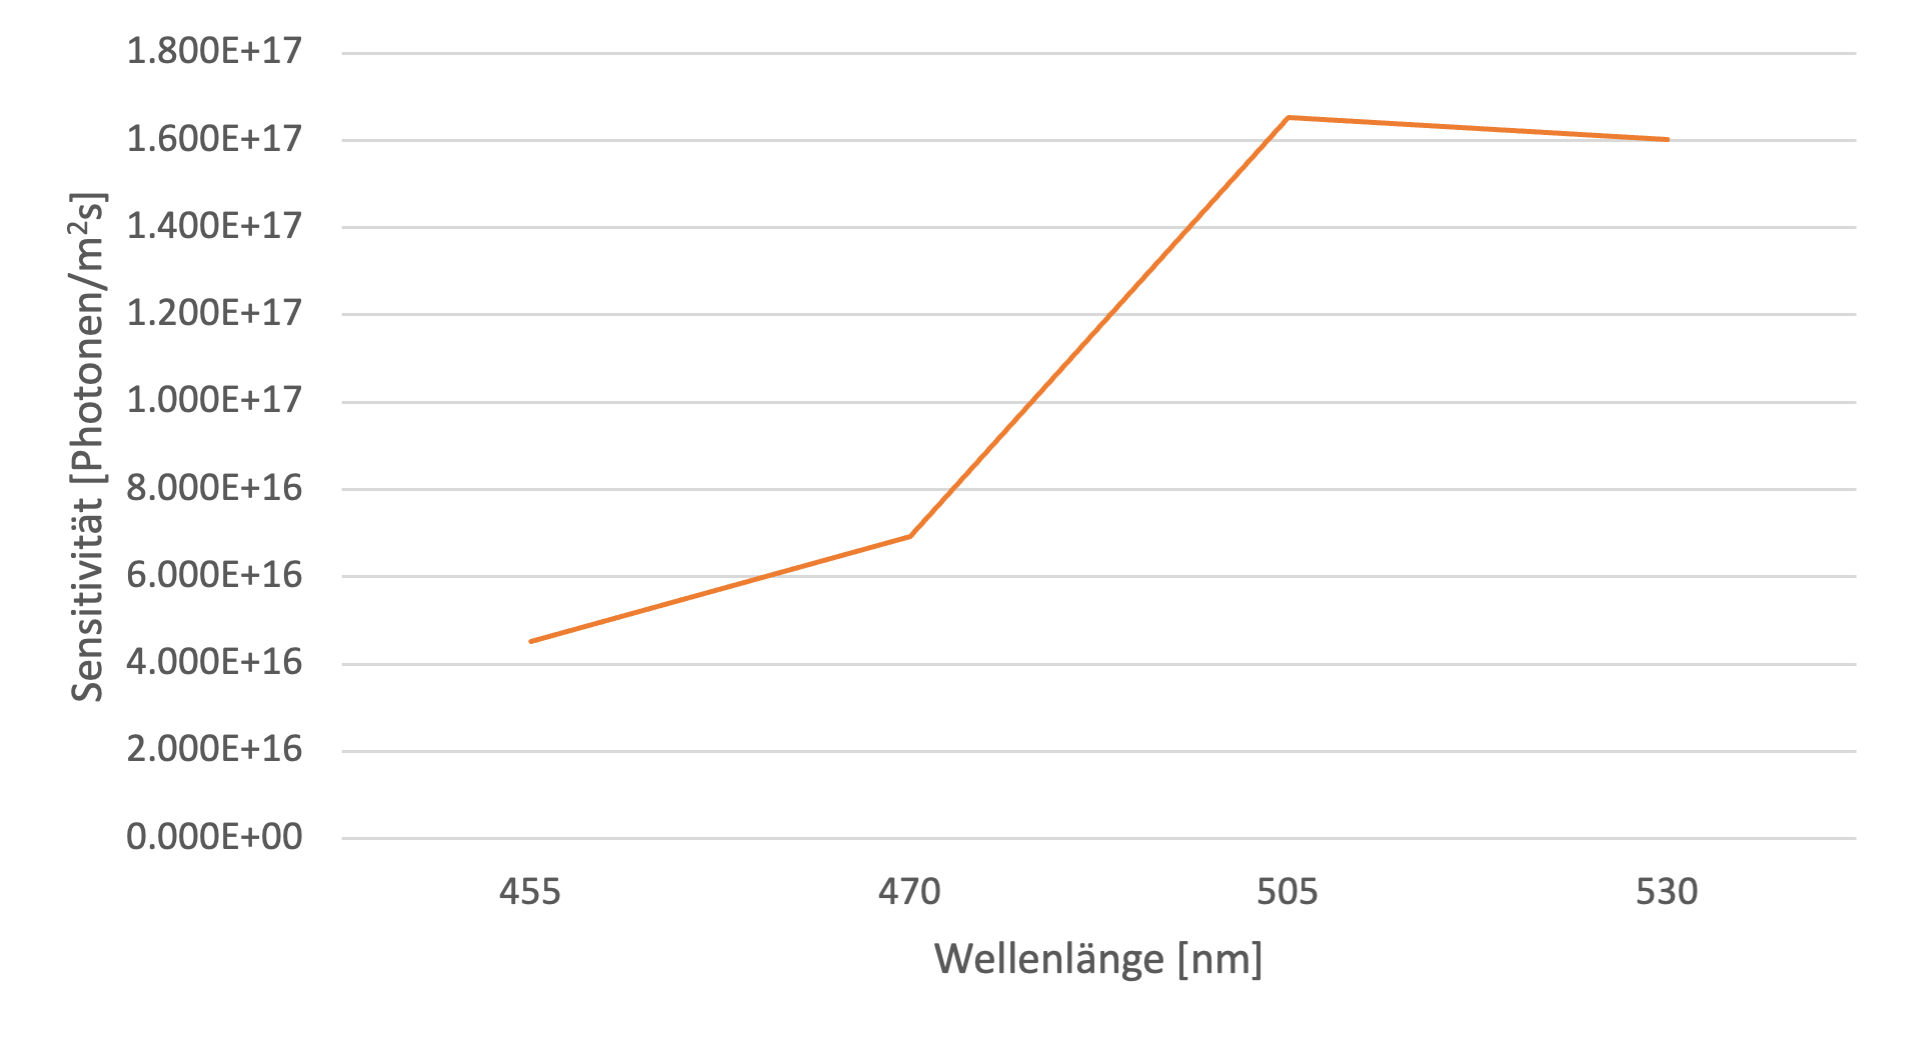
\includegraphics[scale=1]{Picture 6.png}
		\caption{Absorptionsspektrum von nativen eGFP und Puffer bei  $\lambda$ = 350-520 nm. \\
			Puffer dient hier als Referenzprobe\\
			Der Absorptionsmaxima liegt bei $\lambda$ = 490 nm.}
		\label{fig: Aktionsspektrum}
	\end{figure}
	
	\section{Disskusion}
	
	
\end{document}